\documentclass[class=jsarticle, crop=false, dvipdfmx, fleqn]{standalone}
%% preamble for Numerical-structure-analysis report

\input{/Users/User/Documents/Project/TeX/preamble/mypreamble}

%% titles
\title{先端データ解析論 レポート}
\author{37-196360 \quad 森田涼介}


%% setting for listings
\newtcbinputlisting[auto counter]{\reportlisting}[3][]{%
	listing file = {#3},
	listing options = {language=python, style=tcblatex, numbers=left, numberstyle=\tiny},
	listing only,
	breakable,
	toprule at break = 0mm,
	bottomrule at break = 0mm,
	left = 6mm,
	sharp corners,
	drop shadow,
	title = Listings \thetcbcounter : \texttt{#2},
	label = #1,
	}



%% title format
\usepackage{titlesec}
\titleformat{\section}{\LARGE}{宿題\thesection}{0zw}{}
\newcommand{\sectionbreak}{\clearpage}
\titleformat{\subsection}{\Large}{\Alph{subsection})}{0zw}{}

\begin{document}
\section{}

最近傍類似度に対するラプラス固有写像を実装する。

類似度行列を次のように定義する。
\begin{equation}
    W_{i, i'} =
        \begin{cases}
            1 & \text{if } \bm{x}_i \in \mathrm{kNN}(\bm{x}_{i'}) \text{or } \bm{x}_{i'} \in \mathrm{kNN}(\bm{x}_i) \\
            0 & \text{otherwise}
        \end{cases}
\end{equation}
なお,最近傍類似度を考えるので,\(k = 1\)とする。
ラプラス固有写像の埋め込み先\(\bm{\Psi}^\mathrm{T}\)は,
\begin{align}
    & \bm{D} = \mathrm{diag}\qty(\sum_{i'=1}^{n} W_{i, i'}) \\
    & \bm{L} = \bm{D} - \bm{W}
\end{align}
についての固有値問題
\begin{equation}
    \bm{L} \bm{\psi} = \gamma \bm{D} \bm{\psi}
\end{equation}
を解き,
\begin{align}
    & \bm{\Psi}^\mathrm{T} =
        \begin{bmatrix}
            \psi_{n-1} & \psi_{n-2} & \psi_{n-m}
        \end{bmatrix}^\mathrm{T} \\
    & (\gamma_1 \ge \cdots \ge \gamma_n) \qquad \bm{\psi}_i^\mathrm{T} \bm{D} \bm{\psi}_i = 1
\end{align}
とすればよい。

実験では3次元データを2次元に次元削減する。
\pageref{listing:assignment2}ページのListing \ref{listing:assignment2}にプログラムを示した。
結果は図\ref{fig:result}に示した通りである。


\begin{figure}[H]
    \centering
    %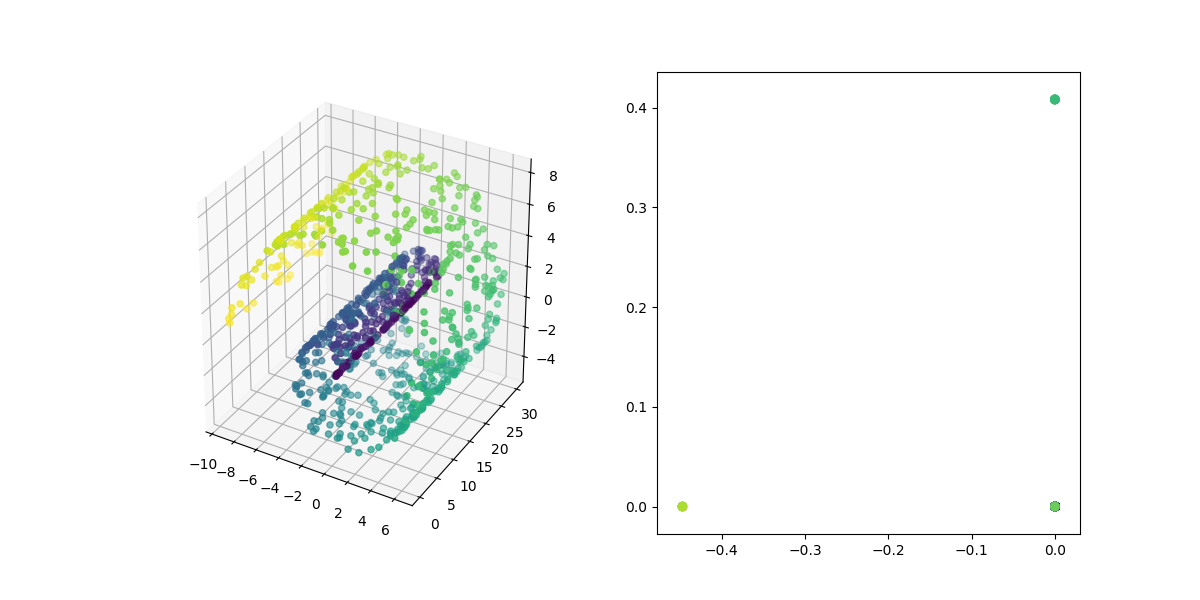
\includegraphics[clip, width=12cm]{../figures/assignment2_result}
    \caption{結果}
    \label{fig:result}
\end{figure}



\end{document}
